%% Pauli frame sampling on four FPGA nodes
%% Author: Nasir Ali, C-DAC Noida

\documentclass[pdflatex,sn-mathphys-num]{sn-jnl}
\pdfgentounicode=1
\input{glyphtounicode}
\usepackage[T1]{fontenc}
\usepackage{lmodern}
\usepackage{graphicx}
\usepackage{multirow}
\usepackage{amsmath,amssymb,amsfonts}
\usepackage{amsthm}
\usepackage[title]{appendix}
\usepackage{xcolor}
\usepackage{textcomp}
\usepackage{manyfoot}
\usepackage{booktabs}
\usepackage[utf8]{inputenc}
\usepackage{algorithm}
\usepackage{algorithmicx}
\usepackage{algpseudocode}
\usepackage{array}
\usepackage{url}
\usepackage{etoolbox}
\AtBeginEnvironment{table}{\small}

\newcommand{\PENDING}[1]{\textcolor{red}{[PENDING: #1]}}
\newcommand{\band}{\mathbin{\&}}
\newcommand{\shr}{\mathbin{\gg}}
% generated by scripts/make_numbers.py
% generated by scripts/make_numbers.py; do not edit
\newcommand{\NumBenchCheckPassed}{12}
\newcommand{\NumBenchCheckTotal}{12}
\newcommand{\NumBenchFile}{batch_20261014_1141.json}
\newcommand{\NumBenchReps}{3}
\newcommand{\NumCosimBatchesA}{4}
\newcommand{\NumCosimBatchesB}{12}
\newcommand{\NumCosimCyclesA}{3{,}281}
\newcommand{\NumCosimCyclesB}{7{,}412}
\newcommand{\NumCosimOverhead}{1.4}
\newcommand{\NumCosimPerBatch}{516.4}
\newcommand{\NumCosimRepPass}{PASS}
\newcommand{\NumCpuAllRep}{140~million}
\newcommand{\NumCpuAllSurfFive}{57.2~million}
\newcommand{\NumCpuAllSurfThree}{124~million}
\newcommand{\NumCpuMaxProcs}{256}
\newcommand{\NumCpuOneRep}{6~million}
\newcommand{\NumCpuOneSurfFive}{724~thousand}
\newcommand{\NumCpuOneSurfThree}{2.84~million}
\newcommand{\NumCpuReps}{3}
\newcommand{\NumDepthFrame}{5}
\newcommand{\NumDepthNoise}{25}
\newcommand{\NumFailedBuilds}{3}
\newcommand{\NumFailingEndpoints}{0}
\newcommand{\NumFirstKernelRep}{865{,}117}
\newcommand{\NumFirstKernelSurfFive}{33{,}587}
\newcommand{\NumFirstKernelSurfThree}{160{,}104}
\newcommand{\NumFirstTierThree}{458}
\newcommand{\NumFirstTierThreeTotal}{458}
\newcommand{\NumFpgaFourRep}{1.16~billion}
\newcommand{\NumFpgaFourSurfFive}{61.4~million}
\newcommand{\NumFpgaFourSurfThree}{296~million}
\newcommand{\NumFpgaOneRep}{289~million}
\newcommand{\NumFpgaOneSurfFive}{15.3~million}
\newcommand{\NumFpgaOneSurfThree}{73.9~million}
\newcommand{\NumFpgaTwoRep}{578~million}
\newcommand{\NumFpgaTwoSurfFive}{30.7~million}
\newcommand{\NumFpgaTwoSurfThree}{148~million}
\newcommand{\NumHazardDistance}{8}
\newcommand{\NumHlsAllIIOne}{1}
\newcommand{\NumHlsDsp}{12}
\newcommand{\NumHlsDspSlr}{0}
\newcommand{\NumHlsFf}{82{,}131}
\newcommand{\NumHlsFfSlr}{9}
\newcommand{\NumHlsFmax}{338}
\newcommand{\NumHlsLut}{145{,}414}
\newcommand{\NumHlsLutSlr}{33}
\newcommand{\NumHostCpu}{AMD EPYC 7742}
\newcommand{\NumHostMemGiB}{504}
\newcommand{\NumHostSockets}{2}
\newcommand{\NumHostThreads}{256}
\newcommand{\NumInstancesPerCard}{2}
\newcommand{\NumKernelMhz}{300}
\newcommand{\NumLanes}{64}
\newcommand{\NumMaxFpgaTemp}{72}
\newcommand{\NumMeasMax}{2{,}048}
\newcommand{\NumModelCardRep}{295~million}
\newcommand{\NumModelCardSurfFive}{15.4~million}
\newcommand{\NumModelCardSurfThree}{74.6~million}
\newcommand{\NumModelFracRep}{98}
\newcommand{\NumModelFracSurfFive}{99}
\newcommand{\NumModelFracSurfThree}{99}
\newcommand{\NumNopsRep}{74}
\newcommand{\NumNopsSurfFive}{16}
\newcommand{\NumNopsSurfThree}{28}
\newcommand{\NumOutMax}{512}
\newcommand{\NumOverFirstRep}{334}
\newcommand{\NumOverFirstSurfFive}{457}
\newcommand{\NumOverFirstSurfThree}{462}
\newcommand{\NumPairs}{32}
\newcommand{\NumPhiloxDsp}{2{,}076}
\newcommand{\NumPhiloxDspCardPct}{46}
\newcommand{\NumPhiloxDspSlr}{69}
\newcommand{\NumProgMax}{8{,}192}
\newcommand{\NumQubitsMax}{128}
\newcommand{\NumRatioAllRep}{8.24}
\newcommand{\NumRatioAllSurfFive}{1.07}
\newcommand{\NumRatioAllSurfThree}{2.39}
\newcommand{\NumRatioOneRep}{193}
\newcommand{\NumRatioOneSurfFive}{84.8}
\newcommand{\NumRatioOneSurfThree}{104}
\newcommand{\NumRepReuses}{51}
\newcommand{\NumRepReusesAtD}{36}
\newcommand{\NumRoutedDspOne}{12}
\newcommand{\NumRoutedDspPct}{0.27}
\newcommand{\NumRoutedFfOne}{61{,}272}
\newcommand{\NumRoutedFfPct}{5.06}
\newcommand{\NumRoutedLutOne}{80{,}941}
\newcommand{\NumRoutedLutPct}{13.76}
\newcommand{\NumScaleEffMax}{100}
\newcommand{\NumScaleEffMin}{100}
\newcommand{\NumScaleFactorMax}{4.00}
\newcommand{\NumScaleFactorMin}{3.99}
\newcommand{\NumSlotsRep}{130}
\newcommand{\NumSlotsSeven}{7{,}035}
\newcommand{\NumSlotsSevenQubits}{97}
\newcommand{\NumSlotsSurfFive}{2{,}489}
\newcommand{\NumSlotsSurfThree}{515}
\newcommand{\NumStimVersion}{1.13.0}
\newcommand{\NumTfImplTime}{2 h 04 min}
\newcommand{\NumTierFiveMaxZ}{1.25}
\newcommand{\NumTierFourMaxZ}{3.12}
\newcommand{\NumTierFourShots}{10{,}223{,}616}
\newcommand{\NumValidationPassed}{all}
\newcommand{\NumWns}{0.003}
\newcommand{\NumXrtVersion}{2.16.204}


\theoremstyle{thmstyleone}
\newtheorem{proposition}{Proposition}

\raggedbottom

\begin{document}

\title[Pauli Frame Sampling on Four FPGA Nodes]{Pauli Frame Sampling on Four FPGA Nodes: A Pipelined Stabilizer
Circuit Sampler for Quantum Error Correction on Alveo U55C Accelerators}

\author*[1]{\fnm{Nasir} \sur{Ali}}\email{nasirali2607@gmail.com}

\affil*[1]{\orgdiv{Embedded Systems Division},
           \orgname{Centre for Development of Advanced Computing},
           \orgaddress{\city{Noida}, \postcode{201307}, \country{India}}}

\abstract{Estimating thresholds and benchmarking decoders for quantum error correction requires sampling very large numbers of
detector outcomes from noisy stabilizer circuits, today mostly with the Stim library on CPUs. We
present a Pauli frame sampler for the AMD Alveo U55C that processes one instruction slot per clock cycle for
\NumLanes{} shots at a time, and we run it on four cards in one host that are treated as independent nodes, as in our
earlier multi FPGA statevector simulator. Three changes remove the bottlenecks of a first single card kernel:
noise masks are produced by a separate pipelined stage from a multiplier free counter based generator, the Pauli frame of up
to \NumQubitsMax{} qubits is updated through a one read, one write pipeline whose hazards the compiler removes by
scheduling, and detectors are folded from a per batch measurement record while the next batch runs. Each card holds \NumInstancesPerCard{} kernel instances in separate super logic regions, and every node, instance
and batch draws its own random stream, so the nodes exchange no data. The kernel is bit exact against a software model in
C simulation, in RTL cosimulation and on every card, and its detector rates and decoded logical error rates agree with
Stim for surface codes up to distance 7. On four cards the sampler delivers \NumFpgaFourSurfFive{} shots per second
for a distance 5 surface code, against \NumCpuOneSurfFive{} for one Stim process and
\NumCpuAllSurfFive{} for \NumCpuMaxProcs{} Stim processes on the host's \NumHostThreads{} hardware threads.
}

\keywords{FPGA, Quantum error correction, Stabilizer circuit simulation, Pauli frame, Multi-FPGA, High-level
synthesis, Alveo U55C, Surface code}

\maketitle

\section{Introduction}\label{sec:intro}

Quantum error correction protects logical information by measuring stabilizers of a code repeatedly and decoding the
resulting detector events. The surface code~\cite{kitaev2003anyons,dennis2002topological,fowler2012surface} is the
leading candidate, and recent experiments have shown logical error rates that fall as the code distance
grows~\cite{google2023scaling,google2025below}. Designing such experiments, estimating thresholds and benchmarking
decoders~\cite{higgott2022pymatching,higgott2025sparse,delfosse2021unionfind} all depend on Monte Carlo sampling:
a noisy stabilizer circuit is sampled millions to billions of times, and every sample (a shot) yields one bit per
detector and per logical observable. The statistical error of a logical error rate $p_L$ estimated from $N$ shots is
about $\sqrt{p_L/N}$, so resolving the small error rates that matter for fault tolerance needs very many shots.

Stim~\cite{gidney2021stim} made this workload fast on CPUs. It computes one noiseless reference sample of the circuit
with a stabilizer tableau~\cite{gottesman1998heisenberg,aaronson2004chp} and then samples noisy shots by propagating
only the Pauli frame~\cite{knill2005noisy}, the deviation of each shot from the reference, through the circuit. A
frame update is a few bitwise operations per gate, applied to many shots packed into one machine word. The work is
therefore regular, branch free and independent between shots: an obvious match for a deeply pipelined hardware
datapath with wide words, and also for many devices working side by side.

This paper treats that observation as a systems question for FPGA accelerators. In earlier work we built a
distributed statevector simulator on four Alveo U55C cards in one host, in which every card is a node that holds a
slice of the state, and amplitudes move between nodes through host memory~\cite{ali2026multifpga}. Treating the cards
as the nodes of a small cluster, with the host acting as interconnect and scheduler, is the model that let four cards
work as one machine there, and it is the model we adopt here.
Pauli frame sampling fits the same node model, with one important difference: shots are independent, so nodes never
need to exchange data. The questions are then how fast one node can run, whether four nodes scale without
interfering through the shared host, and how the result compares with Stim running on all cores of the same host.

A first single card kernel for this workload, which we built earlier in this project and which has not been
published (Section~\ref{sec:first}), validated the approach end to end on hardware but was slower than one Stim process on every circuit tested, because its instruction
loop was not pipelined and each launch sampled only 64 shots. Here we redesign the kernel around the three costs that
dominated it and run it on four nodes. The contributions are:
\begin{itemize}
\item A dataflow kernel that processes one instruction slot per clock cycle for \NumLanes{} shots
(Section~\ref{sec:arch}): a pipelined counter based noise stage, a Pauli frame in a one read, one write memory that
completes every slot two cycles after reading it, and a detector fold stage that works on a per batch measurement
record while the next batch is simulated.
\item A compiler schedule that removes all frame hazards ahead of time: two slots on the same qubit are placed at
least \NumHazardDistance{} slots apart, so the frame pipeline needs no hazard logic and still runs at the full rate
(Section~\ref{sec:frame}). On a distance 5 surface code the schedule adds only its \NumNopsSurfFive{} padding
slots.
\item A node model for independent sampling on several cards, in which every node, kernel instance and batch draws
its own Threefry stream~\cite{salmon2011random123} and the host only launches work and collects results
(Section~\ref{sec:nodes}).
\item A verification chain from a software model through C simulation and RTL cosimulation to every card, closed by
statistical comparison with Stim and by decoded logical error rates up to distance 7
(Sections~\ref{sec:verification} and~\ref{sec:res-correct}).
\item Measurements on one, two and four cards against Stim with one process and with all cores of the same host
(Section~\ref{sec:res-throughput}).
\end{itemize}

Section~\ref{sec:related} reviews related work, Section~\ref{sec:nodes} describes the node model and
Section~\ref{sec:arch} the kernel. Section~\ref{sec:verification} gives the verification method,
Section~\ref{sec:setup} the experimental setup and Section~\ref{sec:results} the results.
Section~\ref{sec:discussion} discusses limits and Section~\ref{sec:conclusions} concludes.

\section{Related work}\label{sec:related}

\paragraph{Stabilizer simulation.} The Gottesman Knill theorem makes Clifford circuits efficiently simulable through
the Heisenberg picture of stabilizer groups~\cite{gottesman1998heisenberg}. Aaronson and Gottesman gave the tableau
algorithm with destabilizers~\cite{aaronson2004chp}, and Anders and Briegel a graph state representation that they found
faster than the tableau algorithm~\cite{anders2006graph}. Stim~\cite{gidney2021stim} combines a tableau simulation of one
reference shot with Pauli frame sampling of all other shots, vectorised over shots with SIMD instructions; it also
derives the detector error model of a circuit, which decoders such as PyMatching consume~\cite{higgott2022pymatching,
higgott2025sparse}. SymPhase accumulates possible Pauli faults as symbolic phases during a single pass over the circuit and draws
samples by substituting values into the symbolic measurement outcomes; its authors report shorter sampling times than
Stim on their benchmarks~\cite{fang2024symphase}. All of these run on CPUs.

\paragraph{Accelerated stabilizer simulation.} Osama, Thanos and Laarman reformulate tableau evolution and
measurement for GPUs in the QuaSARQ simulator; they report speedups of up to 105 times on circuits with up to 180,000
qubits, consistently shorter run times than Stim, and an advantage in many shot sampling on large
workloads~\cite{osama2026gpu}. quEStab extends the tableau to mixed Clifford and non Clifford circuits on several
GPUs~\cite{shin2026questab}. These GPU simulators are built around the tableau of wide circuits; the sampler of this
paper instead streams the Pauli frames of many shots of a small QEC circuit through a fixed pipeline, and its output is
the detector and observable bits that a decoding study consumes. We are not aware of an FPGA implementation of Pauli
frame sampling other than our own first kernel (Section~\ref{sec:first}); searches of Crossref and arXiv for FPGA
based stabilizer, Clifford or Pauli frame simulators found none.

\paragraph{FPGAs for quantum circuit simulation.} FPGA emulation of quantum circuits dates back two
decades~\cite{khalid2004fpga}. Statevector simulators on HBM equipped cards reach 30 qubits on one
card~\cite{tiwari2026fpga30}, and our four card simulator distributes a statevector over the cards of one host and
treats each card as a node~\cite{ali2026multifpga}. Trefoil and Qu-Trefoil distribute much larger states over FPGAs
attached to SATA storage~\cite{niwase2023trefoil,wei2025qutrefoil}. Statevector simulation is limited by memory and by
the exchange of amplitudes between devices; Pauli frame sampling is limited by neither, which is why it scales over
nodes without communication.

\paragraph{FPGAs in quantum error correction.} Most FPGA work in QEC concerns decoding, where latency matters:
lookup table decoders for small codes~\cite{das2022lilliput}, distributed union find decoders~\cite{
delfosse2021unionfind,liyanage2023fpga,liyanage2024distributed}, HeliosNet, which decodes lattice surgery operations
on five FPGAs connected as a network~\cite{liyanage2024multifpga}, the Collision Clustering decoder on FPGA and ASIC
hardware with megahertz decoding rates~\cite{barber2025decoder}, and real time correction for the Shor and Steane
codes~\cite{ali2026qec}. These systems consume syndromes; the sampler of this
paper produces them, for the offline studies that design codes and test decoders. The two are complementary, and a
sampler that runs on the same class of device as a decoder can feed it test data at hardware rates.

\paragraph{High level synthesis.} The kernel is written in C++ and compiled with Vitis HLS~\cite{amd_ug1399}; Cong et
al.\ review the methodology~\cite{cong2011hls}. The design choices below (dataflow stages connected by streams, loops
pipelined to one iteration per cycle, arrays partitioned into registers) are standard HLS constructs; the
contribution is how the sampling algorithm is arranged so that these constructs reach full rate.

\section{FPGA cards as nodes}\label{sec:nodes}

The system is one host with four Alveo U55C cards~\cite{amd_ds978} on PCIe, the same platform as our distributed
statevector simulator~\cite{ali2026multifpga}. As there, each card is a node: it runs its own copy of the kernel, owns
its share of the work, and communicates only with the host. Figure~\ref{fig:nodes} shows the arrangement. What
differs is the work itself. In the statevector simulator a gate on a qubit that indexes the cards needs amplitudes of
other nodes, and the exchange through host memory sets the scaling. In Pauli frame sampling the shots are
independent, so a node needs nothing from any other node. The host's role shrinks to three tasks: compile the circuit
once, load the same program onto every node, and collect the detector and observable bits that the nodes return.

\begin{figure}[t]
\centering
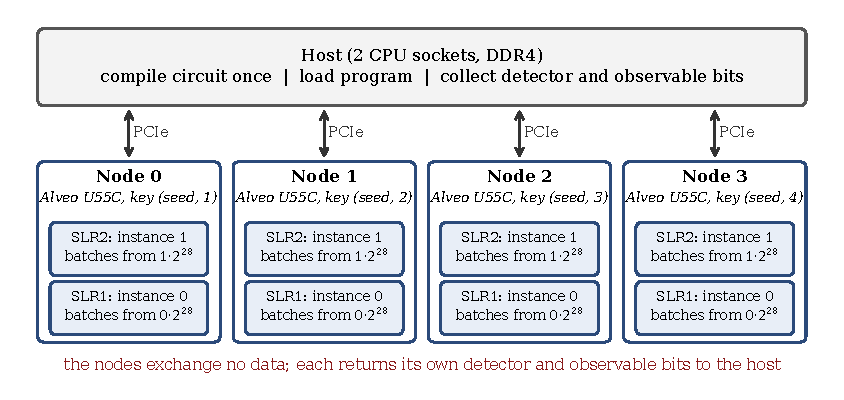
\includegraphics[width=\textwidth]{figures/fig_nodes.pdf}
\caption{Four Alveo U55C cards as nodes of one host. Every card holds \NumInstancesPerCard{} kernel instances, in super
logic regions (SLRs) 1 and 2, each with its own HBM pseudo channels. The host compiles the circuit once, loads the same
program into every instance and receives each instance's detector and observable bits; no data moves between
cards.}\label{fig:nodes}
\end{figure}

\paragraph{Independent random streams.} Independence of the shots only holds if the random numbers of different
nodes are independent. Every noise decision of the kernel is drawn from Threefry4x32-20~\cite{salmon2011random123}, a
counter based generator: its output is a fixed function of a 128 bit counter and a 128 bit key, so any number of
streams can be produced in parallel without shared state, and any single draw can be recomputed in software. Node $c$
uses the key $(s, c+1, 0, 0)$ for a run seed $s$; kernel instance $j$ of a node samples batches $j\cdot 2^{28}$ onwards; and
batch $g$ enters the counter. Two draws of the whole system therefore share a counter and key only if they belong to
the same node, instance, batch, instruction and lane, that is, if they are the same draw. The streams are also
reproducible: the software model of Section~\ref{sec:verification} recomputes the output of any node, instance and
batch from the seed alone, which is how every card is checked bit for bit.

\paragraph{Host side.} One host process per node loads the bitstream, copies the program into every instance once
and then keeps two launches per instance in flight: while one launch runs on the card, the output of the previous
one is copied to host memory. A launch samples a fixed number of batches of \NumLanes{} shots. For measurement, the
processes of all nodes first load their cards and then wait at a common start barrier, so the timed interval of the
system covers the same wall clock window for every node.

\section{Kernel architecture}\label{sec:arch}

\subsection{Pauli frame sampling}\label{sec:frame-sampling}

A Pauli frame assigns to every qubit $q$ and shot a pair of bits $(x_q, z_q)$, the X and Z components of the Pauli
operator by which the noisy shot differs from the noiseless reference. Clifford gates map Pauli operators to Pauli
operators, so the frame is updated by fixed bit rules: H swaps $x_q$ and $z_q$, S sets $z_q \leftarrow z_q \oplus
x_q$, and CX with control $a$ and target $b$ sets $x_b \leftarrow x_b \oplus x_a$ and $z_a \leftarrow z_a \oplus z_b$.
A reset clears the frame of its qubit. A noise channel XORs a random Pauli into the frame. A measurement in the Z basis
flips the shot's outcome relative to the reference exactly when $x_q = 1$, and the analogous rules hold in the X basis
($z_q$) and the Y basis ($x_q \oplus z_q$). A detector is the parity of a set of measurement outcomes whose noiseless
parity is fixed, and the reference parity cancels when two shots are compared; the value of a detector in a shot is
therefore the XOR of the frame flips of its measurements. The kernel never needs the reference sample itself: it emits,
for each detector and logical observable, whether the shot deviates from the noiseless value. This is the quantity
Stim's detector sampler returns~\cite{gidney2021stim}.

With $L$ shots processed together, every frame component of a qubit is an $L$ bit word and every rule above is one
word wide bitwise operation. The kernel uses $L=\NumLanes$ lanes per instance.

\subsection{The first kernel and its costs}\label{sec:first}

The first kernel, built earlier in this project and not published, interprets a stream of instructions one at a
time. Each step fetches a 41 byte
instruction from HBM, applies it to a frame of 64 lanes, draws noise from a 64 lane Philox bank inside the same step,
and on every measurement runs a loop over all 256 detector accumulators to apply the detector mask of that
measurement. Its instruction loop was not pipelined (an attempt to pipeline it reached an initiation interval of 34
cycles and exceeded the resource budget), and each kernel launch sampled 64 shots. These costs, rather than any
property of the algorithm, set its throughput: at a 250~MHz kernel clock it sampled the benchmark circuits of
Section~\ref{sec:setup} at \NumFirstKernelRep{}, \NumFirstKernelSurfThree{} and \NumFirstKernelSurfFive{} shots per
second on one card, below one Stim process on an AMD EPYC 7742. Its output was nevertheless correct: on hardware its
detector rates and its decoded logical error rates (up to distance 5) agreed with Stim, and single fault injection
reproduced all \NumFirstTierThreeTotal{} error mechanisms of the detector error models of three circuits. The kernel described next keeps the instruction semantics of the first
kernel and its software model, and changes how they are executed.

\subsection{Dataflow structure}\label{sec:dataflow}

Figure~\ref{fig:kernel} shows the kernel. At the start of a launch the program and the fold list are copied from HBM
into on chip memory once. Four stages then run concurrently, connected by FIFO streams, over all batches of the
launch:
\begin{enumerate}
\item the noise stage reads one slot per cycle and computes the noise masks of its instruction for all lanes;
\item the frame stage applies one slot per cycle to the Pauli frame and emits the frame flip of every
measurement;
\item the fold stage collects the measurement flips of a batch and computes every detector and observable as the XOR
of its listed measurements;
\item the store stage writes the outputs of every batch to HBM in bursts.
\end{enumerate}
Every loop of every stage is pipelined with an initiation interval of one cycle. The frame stage needs exactly one
cycle per slot, and the other stages need fewer cycles per batch than it does, so a batch of \NumLanes{} shots takes
as many cycles as its program has slots.

\begin{figure}[t]
\centering
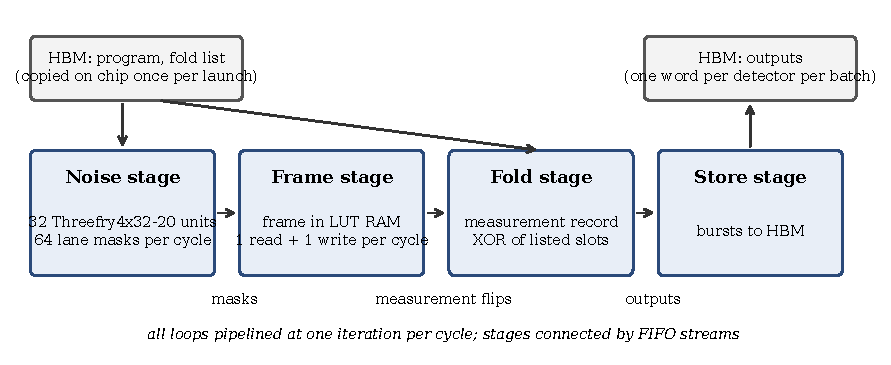
\includegraphics[width=\textwidth]{figures/fig_kernel.pdf}
\caption{Dataflow structure of one kernel instance. The noise stage evaluates \NumPairs{} Threefry4x32-20 units
per cycle; the frame stage keeps the frames in a one read, one write memory and completes every slot two cycles after its
read; the
fold stage keeps a per batch record of measurement flips. Stages are connected by FIFO streams and work on different
instructions or batches at the same time.}\label{fig:kernel}
\end{figure}

\subsection{Program and compiler}\label{sec:program}

The compiler takes a Stim circuit and produces the same instruction list as for the first kernel: broadcast
instructions are split into one instruction per qubit or qubit pair, REPEAT blocks are unrolled, and the measurement
records that every DETECTOR and OBSERVABLE\_INCLUDE refers to are resolved to absolute measurement indices. It then
applies three transformations specific to this kernel. First, qubits are renumbered densely in order of first use:
the generated surface code circuits use sparse qubit indices, and dense numbering lets a distance 7 surface code
(\NumSlotsSevenQubits{} qubits) fit the \NumQubitsMax{} entries of the frame. Second, every measurement receives a slot in
the measurement record of a batch, and the detector and observable definitions become a fold list: for every output in
order, the record slots of its measurements, with the last entry of each output marked. Third, the instructions are
scheduled for the frame pipeline (Section~\ref{sec:frame}). Every slot is encoded in 64 bits: opcode, the 7 bit index of
the qubit it reads and writes, two flags marking the first and the second slot of a two qubit instruction, an 11 bit
record slot and the 32 bit noise threshold $\lfloor p\cdot 2^{32}\rceil$. Table~\ref{tab:programs} lists the compiled programs.

\subsection{Noise stage}\label{sec:noise}

The noise masks of an instruction depend only on the instruction, the lane and the batch, never on the frame. The noise
stage therefore runs ahead of the frame stage and is decoupled from it by a stream. It uses a counter based generator
from the family of Salmon et al.~\cite{salmon2011random123}, whose members pass the TestU01 BigCrush battery: the output
is a fixed function of a 128 bit counter and a key, so the generator has no state to carry and any draw can be
recomputed in software. For an instruction whose (first) slot is $i$, lane $l$ and batch $g$ the stage evaluates
Threefry4x32-20 with counter $(i, \lfloor l/2\rfloor, g, 0)$ and the node's key. One evaluation yields four 32 bit
words; even lanes use the first two and odd lanes the last two, so \NumPairs{} generator units serve \NumLanes{} lanes
per cycle. For lane $l$ the first word $w_0$ decides whether the channel fires ($w_0 < t$ for the threshold $t$) and
the second word $w_1$ selects which Pauli: $w_1 \bmod 3$ for single qubit depolarizing noise and $w_1 \bmod 15$ for two
qubit depolarizing noise, as in the first kernel and its model. The modulo needs no divider: since $16 \equiv 1
\pmod{15}$, a 32 bit word and the sum of its eight hexadecimal digits are congruent modulo 15, the sum is at most 120,
and one more digit sum and a conditional subtraction give the exact residue; $w_1 \bmod 3$ follows from $w_1 \bmod
15$. The twenty Threefry rounds are pipelined, giving the stage a depth of \NumDepthNoise{} cycles at one slot per
cycle.

The first kernel used Philox4x32-10 from the same family, and so did the first versions of this
kernel. Philox multiplies two 32 bit words in each of its ten rounds; \NumPairs{} pipelined Philox units took
\NumPhiloxDsp{} DSP blocks per instance, \NumPhiloxDspSlr\,\% of those of one SLR. Threefry instead uses only
additions, rotations and exclusive ors, which map to ordinary logic and carry chains: an instance needs
\NumHlsDsp{} DSP blocks. Why this mattered is reported in Section~\ref{sec:res-impl}. The software model computes the
same Threefry function; it reproduces the known answer of the Random123 reference for counter and key zero and agrees
with the ThreeFry generator of the randomgen package on random counters and keys.

\subsection{Frame stage and hazard free scheduling}\label{sec:frame}

The frame stage must apply one instruction per cycle to a frame of up to \NumQubitsMax{} qubits, each with two words
of \NumLanes{} bits. We first held the frame in registers, so that a two qubit instruction could read both of its
qubits and write both back in one cycle. That version reached one instruction per cycle in synthesis after the read,
the gate logic and the write back were split into pipeline steps, but its implementation on the card failed: with two instances, the
routed design failed Vivado's verification with conflicting nets after more than five hours of implementation. A
congestion analysis of that design attributes the most congested short range windows to the frame stage, whose
register crossbar (four 128 way selections and write paths into all frame registers) is local and dense, and the
global and long range windows mostly to the noise stage, whose Philox multipliers fill the DSP columns of their
region. The kernel therefore keeps the frame in a small memory with one read
and one write per cycle, implemented in LUT RAM, and gives every slot exactly one frame read and one frame write. A
single qubit instruction occupies one slot. A two qubit instruction occupies two consecutive slots: the first reads
qubit $a$, the second reads qubit $b$, and their new values are written in the two following cycles. In each cycle
the stage reads the qubit of slot $k$ and completes slot $k-2$ from the operands read two and one cycles earlier; for
the first slot of a pair it computes the new values of both qubits, writes $a$ and keeps $b$, which the second slot
writes one cycle later. A valid bit per qubit, cleared at the start of each batch, makes an unwritten qubit read as
zero, so the memory never needs to be cleared. The synthesised frame loop runs at one slot per cycle with a depth of
\NumDepthFrame{} cycles, and the instance needs \NumHlsLutSlr\,\% of the LUTs of one SLR.

The price is a hazard: the result of slot $k$ is written at the end of cycle $k+2$, so a slot that reads a qubit
fewer than three slots after a slot that touched it sees a stale value. The frame stage does not detect this. Instead
the compiler guarantees that it never happens:

\begin{proposition}\label{prop:schedule}
If every two slots that touch a common qubit are at least $D \ge 3$ apart, the frame stage computes the same frame,
measurement flips and outputs as executing the instructions one at a time in slot order.
\end{proposition}

\begin{proof}
Slot $k$ reads its qubit in cycle $k$, and the value of slot $k'$ is written at the end of cycle $k'+2$, so the read
sees the result of every slot $k'\le k-3$ and of no later slot. Every earlier slot on the same qubit has $k'\le k-D\le
k-3$, so the value read is the one the sequential execution would read. For a pair occupying slots $k$ and $k+1$, the
new values are computed in cycle $k+2$ from the operands of both slots, which are correct by the same argument for
each of the two qubits. Slots on disjoint qubits do not interact, and the measurement flip of a slot is computed from
its correct operands.
\end{proof}

The compiler enforces $D=\NumHazardDistance$, more than the three slots needed, as margin for the cycle in which the
synthesised hardware performs the read and the write; RTL cosimulation of the repetition code, in which \NumRepReusesAtD{} of the \NumRepReuses{} reuses
of a qubit are at the minimum distance, confirms that the margin holds. The scheduler fills slots one by one: each slot, or pair of
slots, takes the earliest instruction in compiler order whose qubits were last touched at least $D$ slots before and
whose predecessors on each of its qubits are already placed, or a NOP if there is none. The order of the instructions
on every qubit is unchanged, and instructions on disjoint qubits commute, so the schedule computes the same frame as
the compiler order. The program begins and ends with $D$ NOPs, which write nothing, so that no write or measurement of
one batch reaches past the clear of the valid bits at the start of the next. Two qubit instructions cost two slots,
and NOPs cost slots only when a circuit has too little parallelism: Table~\ref{tab:programs} shows
\NumNopsSurfFive{} NOPs, all of them padding, for the distance 5 surface code, and more for the small repetition
code, whose five qubits cannot fill the slots between reuses.

The scheduler is checked by tests that every two slots on a qubit are at least $D$ apart, that the two slots of a
pair are consecutive, that the program begins and ends with $D$ NOPs, and that the sequence of instructions on every
qubit is identical to the compiler order. A negative control shows that the C simulation of the kernel models the
delayed write: compiled with $D=2$, a circuit whose every instruction depends on the one before produces output that
differs from the software model.

\subsection{Fold and store stages}\label{sec:fold}

The first kernel folded each measurement into the detectors immediately, which needs a read, modify and write of
detector accumulators that two nearby measurements may share. Here the frame stage only sends the flip of every
measurement, tagged with its record slot, to the fold stage, which writes it into a measurement record of the batch.
When all measurements of the batch have arrived, the fold stage walks the fold list once, XORing the record entries
of each output into an accumulator that is emitted at the last entry. The accumulator is the only state carried from
one entry to the next, and the loop runs at one entry per cycle. The fold of batch $g$ overlaps the frame simulation
of batch $g+1$, which needs a FIFO deep enough to hold the measurement flips produced meanwhile. The store stage
writes the outputs of every batch to HBM in bursts: for each batch, one word of \NumLanes{} bits per detector and per
observable, bit $l$ belonging to shot $l$ of the batch.

\subsection{Several instances per card}\label{sec:instances}

The Alveo U55C device has three super logic regions (SLRs); SLR0 also holds the platform's HBM controllers and DMA
engine. A card holds \NumInstancesPerCard{} instances of \NumLanes{} lanes, placed in SLR1 and SLR2 and connected to
their own HBM pseudo channels through the SLR crossings. The
instances of a card run independently, on disjoint batch ranges (Section~\ref{sec:nodes}).

\section{Verification method}\label{sec:verification}

A sampler that is fast but subtly biased is worse than a slow one, because its errors propagate silently into
threshold estimates. The kernel is therefore checked at every level of its implementation against a single software
model, and the model is checked against Stim.

\paragraph{Software model.} The model interprets the compiled program in Python with one boolean frame per qubit and
shot. Its gate, measurement, noise and fold semantics are those of the model of the first kernel, which was validated
against Stim and against single fault injection from Stim's detector error model (Section~\ref{sec:first}); only the
random stream of Section~\ref{sec:noise} is new. Given the program, the seed, the node key and the batch range, the model
produces the exact output words the kernel must produce.

\paragraph{Bit exact levels.} The same comparison is applied at four levels, each catching a different class of
error:
\begin{enumerate}
\item C simulation of the kernel source compiled with g++, for four circuits (repetition code, surface code memory in
the Z and the X basis), two seeds and two batch offsets, one of them near the top of the 32 bit batch counter range. Noiseless circuits must give all zero outputs.
\item The negative control of Section~\ref{sec:frame}, which shows that the C simulation would detect a schedule
violation.
\item RTL cosimulation of the synthesised kernel with Vitis HLS, which runs the generated hardware description,
including the pipelined frame stage and the concurrent dataflow stages: the repetition code, in which \NumRepReusesAtD{} of the
\NumRepReuses{} reuses of a qubit are at the minimum schedule distance, and \NumCosimBatchesA{} and \NumCosimBatchesB{} batches of the
distance 3 surface code, which uses every gate and noise type of the benchmarks.
\item Every kernel instance of every card on hardware, for the three benchmark circuits, with the node key of that
card and batch offsets in two launches.
\end{enumerate}

\paragraph{Statistical levels.} Bit exactness against the model establishes that the hardware computes what the model
computes. Agreement with Stim then establishes that the model samples the right distribution. Two tests are run on
hardware samples. Tier 4 compares the firing rate of every detector and observable with Stim's sampler over
\NumTierFourShots{} shots per side for the three benchmark circuits, using a two proportion $z$ score per output and
requiring $|z|<5$ for all of them. Tier 5 decodes hardware samples and Stim samples of rotated surface code memory
experiments with distance $d=3,5,7$ ($d$ rounds) and physical error rate $p=0.001,0.003,0.01$ with the same
PyMatching~\cite{higgott2022pymatching,higgott2025sparse} matcher, built from Stim's detector error model, and requires
the logical error rates to agree with $|z|<5$. Distance 7 could not be run on the first kernel, which lacked the
qubit renumbering.

\section{Experimental setup}\label{sec:setup}

\paragraph{Platform.} The host has two \NumHostCpu{} processors with \NumHostThreads{} hardware threads in total and
\NumHostMemGiB{}~GiB of memory, and four Alveo U55C cards~\cite{amd_ds978} with the platform
\texttt{xilinx\_u55c\_gen3x16\_xdma\_base\_3}, each in its own PCIe slot, driven by XRT~\NumXrtVersion{}~\cite{amd_xrt}.
The kernel was synthesised with Vitis HLS 2023.2~\cite{amd_ug1399} and linked with \texttt{v++} 2023.2 at a kernel
clock of \NumKernelMhz{}~MHz, with \NumInstancesPerCard{} instances per card.

\paragraph{Circuits.} The three benchmark circuits are those used to evaluate the first kernel
(Section~\ref{sec:first}), generated by Stim: a repetition code memory experiment with distance 3 and 3 rounds (data and measurement noise
0.05), and rotated surface code memory experiments in the Z basis with distance 3 and 3 rounds and with distance 5
and 5 rounds, each with data depolarization before every round, measurement flips, depolarization after every Clifford
gate and reset flips, all at probability 0.02. Table~\ref{tab:programs} lists the compiled programs.

\paragraph{CPU baseline.} Stim~\NumStimVersion{} runs on the same host. A Stim process compiles the detector sampler of
the circuit (not timed) and then samples bit packed detector and observable data; the rate is the number of shots
divided by the sampling time. Stim's sampler uses one thread per process, so the parallel baseline starts $P$
processes behind a common barrier, each sampling its own share with its own seed, and divides the total number of
shots by the time of the slowest process. We report $P=1$ and $P$ up to \NumCpuMaxProcs{}, the number of hardware
threads of the host; every point is the median of \NumCpuReps{} runs, taken while the cards were idle.

\paragraph{FPGA measurement.} For each circuit and for one, two and four cards, one host process per card loads its
card and the program, waits at the common barrier, and then runs a fixed number of launches of 4096 batches per
instance, each launch's output copied back to host memory before it counts. The system rate is the total number of
shots of all cards divided by the interval from the earliest start to the latest end of the timed loops. Each
configuration is repeated \NumBenchReps{} times and the median is reported. Before any timing, every instance of every
card passes the bit exact check of Section~\ref{sec:verification}. Card temperatures are recorded before and after
every configuration.

\section{Results}\label{sec:results}

\subsection{Compiled programs}\label{sec:res-programs}

Table~\ref{tab:programs} lists the compiled programs. The schedule of Section~\ref{sec:frame} adds no NOPs beyond
the padding for the distance 5 and 7 surface codes, whose layers hold many independent instructions; their slot
counts exceed the instruction counts by the second slots of the two qubit instructions. The distance 3
surface code needs a few NOPs and the repetition code, with five qubits, needs most of its slots as NOPs; both
programs are short, so a batch still takes only a few hundred cycles.

\begin{table}[t]
\caption{Compiled programs. Instructions excludes the NOPs inserted by the schedule. Slots, the cycles per batch of
the frame stage, counts one slot per single qubit instruction, two per two qubit instruction and one per NOP.
Columns: qubits after renumbering, instructions, two qubit (2q) instructions, NOPs, slots, measurements,
outputs (detectors plus observables) and fold entries.}\label{tab:programs}
% generated by scripts/make_numbers.py
\begin{tabular}{@{}lrrrrrrrr@{}}
\toprule
Circuit & Qubits & Instr. & 2q & NOPs & Slots & Meas. & Out. & Fold \\
\midrule
Repetition code, $d=3$ & 5 & 44 & 12 & 74 & 130 & 9 & 9 & 17 \\
Surface code, $d=3$ & 17 & 343 & 144 & 28 & 515 & 33 & 25 & 55 \\
Surface code, $d=5$ & 49 & 1{,}673 & 800 & 16 & 2{,}489 & 145 & 121 & 261 \\
Surface code, $d=7$ & 97 & 4{,}667 & 2{,}352 & 16 & 7{,}035 & 385 & 337 & 715 \\
\botrule
\end{tabular}

\end{table}

\subsection{Synthesis and implementation}\label{sec:res-impl}

All loops of the kernel were scheduled by Vitis HLS with an initiation interval of one cycle, and HLS estimated a
maximum clock of \NumHlsFmax{}~MHz for a target of 300~MHz. Placing and routing the kernel on the card was the
difficult step. Table~\ref{tab:builds} lists every implementation run, each with two instances at 300~MHz. The
\NumFailedBuilds{} runs with the Philox noise stage all failed Vivado's verification of the routed design with
conflicting nets, after about five hours each: first with the frame in registers, then with the frame in LUT RAM, and
then also with a placement directive that spreads logic to relieve congestion. The congestion analysis of the first
run (Section~\ref{sec:frame}) explains the pattern: removing the register crossbar removed the short range hot spots,
but the noise stage with \NumPhiloxDsp{} DSP blocks per instance still filled the DSP columns of its region, and in
all three runs every one of the ten conflicting nets that Vivado lists lay in the instance placed in SLR0, which it
shares with the platform's HBM and DMA logic. Replacing Philox by Threefry removed the DSP demand (\NumHlsDsp{} DSP blocks per instance), and the
instances were moved to SLR1 and SLR2. With both changes the design routed: the placer no longer reported the
design as congested, and the run with the standard placement directive met timing at 300~MHz with a worst negative
slack of \NumWns{}~ns after \NumTfImplTime{} of implementation, less than half the time of each failed run. The
parallel run with the spreading directive was stopped once this result was available.

\begin{table}[t]
\caption{Implementation runs of the kernel on the Alveo U55C, two instances at a 300~MHz target. Frame: frame stage
storage. Generator: Philox4x32-10 or Threefry4x32-20. SLRs: the regions of the two instances. Placement: Vivado
directive ExtraTimingOpt (timing) or AltSpreadLogic\_high (spread). DSP: DSP blocks per instance (HLS). Time: Vivado
placement and routing. All runs used the
same post route optimisation settings.}\label{tab:builds}
% generated by scripts/make_numbers.py
\begin{tabular}{@{}llllrrl@{}}
\toprule
Frame & Generator & SLRs & Placement & DSP & Time & Outcome \\
\midrule
registers & Philox & 0, 1 & timing & 2{,}076 & 5~h 18~min & routing failed \\
LUT RAM & Philox & 0, 1 & timing & 2{,}076 & 4~h 55~min & routing failed \\
LUT RAM & Philox & 0, 1 & spread & 2{,}076 & 5~h 23~min & routing failed \\
LUT RAM & Threefry & 1, 2 & timing & 12 & 2~h 04~min & bitstream \\
LUT RAM & Threefry & 1, 2 & spread & 12 & stopped & stopped \\
\botrule
\end{tabular}

\end{table}

Table~\ref{tab:resources} compares the HLS estimate of one instance with the routed design. The HLS estimate of logic is
conservative: a routed instance uses \NumRoutedLutOne{} LUTs
against \NumHlsLut{} estimated. The routed design runs at \NumKernelMhz{}~MHz with a worst negative slack of
\NumWns{}~ns.

\begin{table}[t]
\caption{Resources of the kernel. HLS: estimate for one instance, in percent of one SLR. Routed: one instance, and
all \NumInstancesPerCard{} instances of a card in percent of the resources available to user logic, from the post
route utilisation report.}\label{tab:resources}
% generated by scripts/make_numbers.py
\begin{tabular}{@{}lrrrr@{}}
\toprule
Resource & HLS, one instance & \% SLR & Routed, one instance & Routed, card (\% budget) \\
\midrule
LUT & 145{,}414 & 33 & 80{,}941 & 161{,}975 (13.76) \\
FF & 82{,}131 & 9 & 61{,}272 & 122{,}546 (5.06) \\
DSP & 12 & 0 & 12 & 24 (0.27) \\
\botrule
\end{tabular}

\end{table}

RTL cosimulation of the distance 3 surface code took \NumCosimCyclesA{} cycles for \NumCosimBatchesA{} batches and
\NumCosimCyclesB{} cycles for \NumCosimBatchesB{}, that is \NumCosimPerBatch{} cycles per additional batch for a
program of \NumSlotsSurfThree{} slots. The four stages keep pace with each other: the frame stage completes one slot
per cycle, and a batch costs \NumCosimOverhead{} cycles more than its slots.

\subsection{Correctness on hardware}\label{sec:res-correct}

Every kernel instance of every card produced output bit identical to the software model for the three benchmark
circuits (\NumBenchCheckPassed{} of \NumBenchCheckTotal{} card and circuit checks). Table~\ref{tab:tier4} gives the
Tier 4 comparison with Stim and Table~\ref{tab:ler} the Tier 5 logical error rates. All outputs of all circuits agree
with Stim within the $5\sigma$ bound (largest $|z|$ \NumTierFourMaxZ{}), and the decoded logical error rates of
hardware and Stim samples agree at every distance and error rate (largest $|z|$ \NumTierFiveMaxZ{}). The rates show
the expected behaviour of the surface code: below threshold the logical error rate falls with distance, at
$p=0.01$ it rises.

\begin{table}[t]
\caption{Tier 4: detector and observable firing rates of hardware samples against Stim. The largest two proportion
$|z|$ over all outputs of a circuit is reported.}\label{tab:tier4}
% generated by scripts/make_numbers.py
\begin{tabular}{@{}lrrr@{}}
\toprule
Circuit & FPGA shots & Stim shots & max $|z|$ \\
\midrule
Repetition code, $d=3$ & 10{,}223{,}616 & 10{,}000{,}000 & 1.43 \\
Surface code, $d=3$ & 10{,}223{,}616 & 10{,}000{,}000 & 3.12 \\
Surface code, $d=5$ & 10{,}223{,}616 & 10{,}000{,}000 & 2.74 \\
\botrule
\end{tabular}

\end{table}

\begin{table}[t]
\caption{Tier 5: logical error rates (LER) of rotated surface code memory experiments, hardware samples against Stim
samples, both decoded by the same PyMatching matcher.}\label{tab:ler}
% generated by scripts/make_numbers.py
\begin{tabular}{@{}rrrrrr@{}}
\toprule
$d$ & $p$ & Shots & FPGA LER & CPU Stim LER & $z$ \\
\midrule
3 & 0.001 & 1{,}048{,}576 & 7.753e-04 & 7.734e-04 & $+0.05$ \\
3 & 0.003 & 1{,}048{,}576 & 6.518e-03 & 6.616e-03 & $-0.87$ \\
3 & 0.010 & 1{,}048{,}576 & 5.939e-02 & 5.908e-02 & $+0.97$ \\
5 & 0.001 & 1{,}048{,}576 & 1.402e-04 & 1.373e-04 & $+0.18$ \\
5 & 0.003 & 1{,}048{,}576 & 3.340e-03 & 3.286e-03 & $+0.67$ \\
5 & 0.010 & 1{,}048{,}576 & 8.339e-02 & 8.377e-02 & $-0.99$ \\
7 & 0.001 & 1{,}048{,}576 & 1.621e-05 & 2.289e-05 & $-1.09$ \\
7 & 0.003 & 1{,}048{,}576 & 1.466e-03 & 1.533e-03 & $-1.25$ \\
7 & 0.010 & 1{,}048{,}576 & 1.034e-01 & 1.032e-01 & $+0.39$ \\
\botrule
\end{tabular}

\end{table}

\subsection{Throughput on one, two and four nodes}\label{sec:res-throughput}

Table~\ref{tab:throughput} and Figure~\ref{fig:throughput} give the measured sampling rates. One card with
\NumInstancesPerCard{} instances samples the distance 5 surface code at \NumFpgaOneSurfFive{} shots per second, and four
cards at \NumFpgaFourSurfFive{}. Going from one to four nodes multiplies the rate by \NumScaleFactorMin{} to
\NumScaleFactorMax{} over the three circuits, that is, the nodes scale linearly: they share nothing but the host,
and at these output volumes the host side (launching, copying results to host memory, synchronising the processes)
does not limit the rate. The per card rates within a run differ by less than one percent. The FPGA temperatures read before and after
every configuration were at most \NumMaxFpgaTemp{}~\textdegree C.

\begin{table}[t]
\caption{Sampling rates in shots per second (median of \NumBenchReps{} runs) on one, two and four cards. $S_4$: four
card rate over one card rate. $R_1$, $R_{\mathrm{all}}$: four card rate over Stim on the same host with one process
and with \NumCpuMaxProcs{} processes (Table~\ref{tab:cpu}). All rates count only shots whose outputs have reached host
memory.}\label{tab:throughput}
% generated by scripts/make_numbers.py
\begin{tabular}{@{}lrrrrrr@{}}
\toprule
Circuit & 1 card & 2 cards & 4 cards & $S_4$ & $R_1$ & $R_{\mathrm{all}}$ \\
\midrule
Repetition code, $d=3$ & 289{,}230{,}495 & 577{,}517{,}899 & 1{,}155{,}366{,}309 & 3.99$\times$ & 193$\times$ & 8.24$\times$ \\
Surface code, $d=3$ & 73{,}912{,}169 & 147{,}798{,}429 & 295{,}658{,}952 & 4.00$\times$ & 104$\times$ & 2.39$\times$ \\
Surface code, $d=5$ & 15{,}338{,}202 & 30{,}687{,}981 & 61{,}359{,}029 & 4.00$\times$ & 84.8$\times$ & 1.07$\times$ \\
\botrule
\end{tabular}

\end{table}

\begin{figure}[t]
\centering
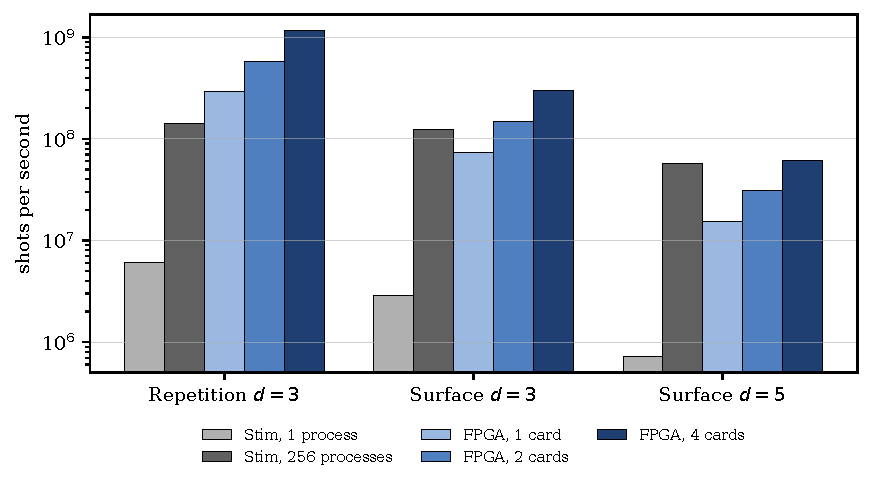
\includegraphics[width=0.85\textwidth]{figures/fig_throughput.pdf}
\caption{Sampling rate of the three benchmark circuits on one, two and four cards, and of Stim with one process and
with all hardware threads of the host. Logarithmic scale.}\label{fig:throughput}
\end{figure}

\begin{table}[t]
\caption{Stim~\NumStimVersion{} on the host: shots per second with $P$ concurrent processes.}\label{tab:cpu}
% generated by scripts/make_numbers.py
\begin{tabular}{@{}lrrrrr@{}}
\toprule
Circuit & 1 proc. & 16 proc. & 64 proc. & 128 proc. & 256 proc. \\
\midrule
Repetition code, $d=3$ & 5{,}999{,}732 & 60{,}814{,}996 & 84{,}704{,}275 & 100{,}987{,}950 & 140{,}258{,}256 \\
Surface code, $d=3$ & 2{,}841{,}093 & 35{,}270{,}693 & 65{,}480{,}163 & 78{,}332{,}218 & 123{,}750{,}688 \\
Surface code, $d=5$ & 723{,}625 & 10{,}181{,}623 & 26{,}614{,}558 & 35{,}169{,}041 & 57{,}200{,}963 \\
\botrule
\end{tabular}

\end{table}

Against one Stim process, the four node system is faster by the factors in Table~\ref{tab:throughput}
(\NumRatioOneSurfFive{} times for the distance 5 surface code). The more demanding comparison is with Stim on all
\NumHostThreads{} hardware threads of the same host: there the four node system reaches \NumRatioAllSurfFive{} times
the CPU rate for the distance 5 surface code, \NumRatioAllSurfThree{} times for the distance 3 surface code and
\NumRatioAllRep{} times for the repetition code. Stim's rate grows less than linearly with the number of processes
(Table~\ref{tab:cpu}); we did not investigate the cause on this host.

\subsection{Comparison with the first kernel and with the cycle model}\label{sec:res-first}

On one card the first kernel sampled the three circuits at \NumFirstKernelRep{}, \NumFirstKernelSurfThree{} and
\NumFirstKernelSurfFive{} shots per second (Section~\ref{sec:first}), measured at a 250~MHz kernel clock on the
project's build host, whose CPU is the same model. The new kernel on one card is faster by factors of
\NumOverFirstRep{}, \NumOverFirstSurfThree{} and \NumOverFirstSurfFive{}. The cycle count of the kernel predicts the
rate of a card from the program alone: an instance delivers \NumLanes{} shots per batch, and a batch takes as many
cycles as the largest of its slot count, its measurement and fold work, and its output count, so a card should
sample at \NumModelCardRep{}, \NumModelCardSurfThree{} and \NumModelCardSurfFive{} shots per second. The measured one
card rates are \NumModelFracRep\,\%, \NumModelFracSurfThree\,\% and \NumModelFracSurfFive\,\% of these predictions; the
remainder is launch overhead and the copy of results to host memory, which weigh most for the short repetition code
program.

\section{Discussion}\label{sec:discussion}

\paragraph{What changed.} The first kernel and the new one execute the same instructions with the same frame
semantics and the same noise decision rules; they differ in the counter based generator that supplies the random
words, and in where the work happens: noise generation moved off the critical loop into its own
pipelined stage, frame hazards moved from hardware into the compiler's schedule, detector folding moved into a stage
that overlaps the next batch, and the cost of a launch is shared by thousands of batches instead of one. Each of these
is a standard technique; together they turn the interpreter of the first kernel into a pipeline whose rate the
compiled program alone determines.

\paragraph{Nodes without communication.} Our distributed statevector simulator on the same four cards spends much of
its time exchanging amplitudes through host memory, and more cards add capacity there rather than
speed~\cite{ali2026multifpga}. Sampling is the opposite case: with independent random streams per node the nodes do
not interact, and the four card rate is four times the one card rate (Table~\ref{tab:throughput}). The node model carries over
unchanged; what decides scaling is whether the workload needs data from other nodes. For workloads of this kind,
more cards in a host, or hosts with cards, add rate in proportion until the host can no longer collect the output.

\paragraph{Routability as the limit.} The synthesis estimates were never the obstacle: every version of the kernel that
was implemented reached one slot per cycle and an estimated clock above the 300~MHz target. What decided between a working and a
failing design was routing, and the cause was density rather than size: the failed designs used \NumPhiloxDspCardPct\,\%
of the DSP blocks available to user logic but packed them into the DSP columns of the regions they occupied, and
the conflicting nets of every failed run lay in the instance that shared SLR0 with the platform logic. A generator
built from adders and rotations, which spreads over ordinary logic, and the move away from SLR0 turned five hour runs
that failed into a two hour run that met timing. For HLS designs that replicate arithmetic units in
parallel, we found the placement of those units on the device to matter as much as their number.

\paragraph{Limits of the kernel.} The frame memory holds \NumQubitsMax{} qubits after renumbering, enough for the
rotated surface code up to distance 7 (\NumSlotsSevenQubits{} qubits) but not distance 9. The program memory holds
\NumProgMax{} slots, the measurement record \NumMeasMax{} measurements and the output stage \NumOutMax{} detectors and
observables. Larger codes need wider limits; the frame memory grows linearly with the qubit count, and the program
and record memories are on chip block RAM. The instruction set covers the gates, measurements, resets and noise channels
of the generated memory experiments (H, S, CX, CZ, SWAP, measurement and reset in three bases, measure and reset,
single qubit Pauli errors, single and two qubit depolarizing noise); other Clifford gates, correlated errors and
Pauli product measurements would need further opcodes. Like the first kernel, it uses the frame semantics that
follow from a Clifford circuit; it does not handle non Clifford gates.

\paragraph{Limits of the comparison.} The CPU baseline is Stim's own detector sampler with one process per hardware
thread, which is how Stim is used for large sampling campaigns; a multi threaded sampler built on Stim might do better
on the same CPU. The comparison concerns sampling only: compiling the circuit, deriving the detector error model and
decoding are done on the host in both cases and are not timed. Energy was not compared, because the host provides no
power measurement of the CPU that would match the board power readings of the cards. The repetition code has only five qubits, so
most slots of its program are NOPs that keep reuses of a qubit apart (Table~\ref{tab:programs}); its rate reflects
the schedule more than the circuit, and the larger circuits are the more representative ones.

\paragraph{Embedded use.} The kernel needs no host interaction while a launch runs and its output is a stream of
detector words. The same pipeline could therefore feed a decoder on the same device or on a device next to it,
replacing recorded test data with live samples at hardware rate, which would make the sampler a test source for the
FPGA decoders of Section~\ref{sec:related}. We have not built that combination.

\section{Conclusions}\label{sec:conclusions}

We presented a Pauli frame sampler for stabilizer circuits that processes one instruction slot per clock cycle for
\NumLanes{} shots per kernel instance, and ran it on four Alveo U55C cards treated as independent nodes of one host. A pipelined
counter based noise stage, a one read, one write frame pipeline whose hazards the compiler schedules away, and a
detector fold that overlaps the next batch remove the costs that made the first kernel slower than one CPU process. The kernel is bit
exact against its software model in C simulation, in RTL cosimulation and on every card, and its samples agree with
Stim in detector rates and in decoded logical error rates up to distance 7. On four nodes it samples the distance 5
surface code at \NumFpgaFourSurfFive{} shots per second, \NumRatioOneSurfFive{} times one Stim process and
\NumRatioAllSurfFive{} times Stim on all \NumHostThreads{} hardware threads of the host.

The routed design with two instances occupies \NumRoutedLutPct\,\% of the LUTs available to user logic and almost
no DSP blocks, which leaves room for more instances per card. The next steps are such wider configurations, wider
limits for larger codes, and a direct connection of the sampler to an FPGA decoder so that decoders can be tested
with live samples.


\backmatter

\bmhead{Acknowledgments}
This work was funded by the Ministry of Electronics and Information Technology (MeitY), Government of India. The
research was conducted at the C-DAC Noida Centre under the supervision of Mr. Abhishek Tiwari, Scientist F, Embedded
Systems Division, C-DAC Noida. We thank the developers of Stim and PyMatching, on which the validation of this work
depends.

\section*{Declarations}

\textbf{Funding.} This work was funded by the Ministry of Electronics and Information Technology (MeitY), Government of
India.

\textbf{Conflict of interest.} The author declares no competing interests.

\textbf{Ethics approval and consent to participate.} Not applicable.

\textbf{Consent for publication.} Not applicable.

\textbf{Data availability.} The raw measurement records that support the findings of this study (one JSON file per
run with timestamps, code revision, bitstream hash and card identifiers), the benchmark circuits and the scripts that
generate every table and figure from them are available from the corresponding author on reasonable request.

\textbf{Author contribution.} N.~Ali designed and implemented the HLS kernel, the compiler, the host runtime and the
validation suite, carried out the measurements and wrote the manuscript.

\bibliography{references}

\end{document}
